% Options for packages loaded elsewhere
\PassOptionsToPackage{unicode}{hyperref}
\PassOptionsToPackage{hyphens}{url}
\PassOptionsToPackage{dvipsnames,svgnames,x11names}{xcolor}
%
\documentclass[
  11pt,
  a4paper,
]{article}
\usepackage{amsmath,amssymb}
\usepackage{iftex}
\ifPDFTeX
  \usepackage[T1]{fontenc}
  \usepackage[utf8]{inputenc}
  \usepackage{textcomp} % provide euro and other symbols
\else % if luatex or xetex
  \usepackage{unicode-math} % this also loads fontspec
  \defaultfontfeatures{Scale=MatchLowercase}
  \defaultfontfeatures[\rmfamily]{Ligatures=TeX,Scale=1}
\fi
\usepackage{lmodern}
\ifPDFTeX\else
  % xetex/luatex font selection
\fi
% Use upquote if available, for straight quotes in verbatim environments
\IfFileExists{upquote.sty}{\usepackage{upquote}}{}
\IfFileExists{microtype.sty}{% use microtype if available
  \usepackage[]{microtype}
  \UseMicrotypeSet[protrusion]{basicmath} % disable protrusion for tt fonts
}{}
\makeatletter
\@ifundefined{KOMAClassName}{% if non-KOMA class
  \IfFileExists{parskip.sty}{%
    \usepackage{parskip}
  }{% else
    \setlength{\parindent}{0pt}
    \setlength{\parskip}{6pt plus 2pt minus 1pt}}
}{% if KOMA class
  \KOMAoptions{parskip=half}}
\makeatother
\usepackage{xcolor}
\usepackage{longtable,booktabs,array}
\usepackage{calc} % for calculating minipage widths
% Correct order of tables after \paragraph or \subparagraph
\usepackage{etoolbox}
\makeatletter
\patchcmd\longtable{\par}{\if@noskipsec\mbox{}\fi\par}{}{}
\makeatother
% Allow footnotes in longtable head/foot
\IfFileExists{footnotehyper.sty}{\usepackage{footnotehyper}}{\usepackage{footnote}}
\makesavenoteenv{longtable}
\usepackage{graphicx}
\makeatletter
\def\maxwidth{\ifdim\Gin@nat@width>\linewidth\linewidth\else\Gin@nat@width\fi}
\def\maxheight{\ifdim\Gin@nat@height>\textheight\textheight\else\Gin@nat@height\fi}
\makeatother
% Scale images if necessary, so that they will not overflow the page
% margins by default, and it is still possible to overwrite the defaults
% using explicit options in \includegraphics[width, height, ...]{}
\setkeys{Gin}{width=\maxwidth,height=\maxheight,keepaspectratio}
% Set default figure placement to htbp
\makeatletter
\def\fps@figure{htbp}
\makeatother
\setlength{\emergencystretch}{3em} % prevent overfull lines
\providecommand{\tightlist}{%
  \setlength{\itemsep}{0pt}\setlength{\parskip}{0pt}}
\setcounter{secnumdepth}{5}
\usepackage[T1]{fontenc}
\usepackage{libertinus}
\DeclareUnicodeCharacter{2212}{\textminus}
\usepackage{microtype}
\usepackage{xurl}
\usepackage[margin=1in]{geometry}
\usepackage{booktabs}
\usepackage{etoolbox}
\AtBeginEnvironment{longtable}{\small}
\setlength{\LTcapwidth}{\textwidth}
\usepackage{caption}
\captionsetup{font=small,labelfont=bf}
\setlength{\emergencystretch}{2em}
\usepackage{float}
\floatplacement{figure}{H}
\ifLuaTeX
  \usepackage{selnolig}  % disable illegal ligatures
\fi
\usepackage{bookmark}
\IfFileExists{xurl.sty}{\usepackage{xurl}}{} % add URL line breaks if available
\urlstyle{same}
\hypersetup{
  pdftitle={Where the histories come from},
  pdfauthor={Leo Lilley},
  colorlinks=true,
  linkcolor={black},
  filecolor={Maroon},
  citecolor={Blue},
  urlcolor={black},
  pdfcreator={LaTeX via pandoc}}

\title{Where the histories come from}
\usepackage{etoolbox}
\makeatletter
\providecommand{\subtitle}[1]{% add subtitle to \maketitle
  \apptocmd{\@title}{\par {\large #1 \par}}{}{}
}
\makeatother
\subtitle{Five post-training cycles and two prompts on a Gemma 4 coding
agent, with every step a verified record}
\author{Leo Lilley}
\date{November 2026}

\begin{document}
\maketitle
\begin{abstract}
Fine-tuning a small coding agent on a larger agent's verified runs
lowered its held-out loss and made it loop. We ran five post-training
cycles on a Gemma 4 agent in the competition's unchanged harness, each
training a LoRA on the small 4-bit E4B model, with every step a
checkable record and each adoption decision made by a rule written
before the evidence; none was adopted. The four adapters trained on the
31B agent's verified histories repeated their previous tool call on 28
to 35\% of calls within the call budget against the base's 3\%; their
task scores, 0 or 1 of 16 against 2, sit inside rerun noise. The loop
deepens itself: an adapter starts a repeat on 7\% of calls and, five
identical calls in, continues 99\% of the time. A frontier swap, which
cuts a recorded history before one call and hands it to another model
for that call only, crosses weights with history: on a looping history
the adapter that wrote it repeats 50\% of the time, another adapter 18\%
and the base 5\%; on clean histories written by the base or the 31B all
repeat on 3\% or less. The 31B joins an established loop in 15 of 17
states, all from one task, and one round of its labels did not stop the
looping. An adapter trained on the learner's own resolved rollouts did
not loop and did not gain; a pre-registered control trained on the 31B's
histories at the same size and settings looped at 28\% within budget.
Two prompt arms did not move the score. We close with a hypothesis the
one-model rule excludes: an agent that switches models per step.
\end{abstract}

\section{Introduction}\label{introduction}

We ran a post-training loop under one discipline: every input selected
by a stated rule, every transformation reproducible from recorded files,
every adoption decision fixed before its evidence. Nothing we trained
helped, so the question the cycles can answer is what decides whether
post-training harms or does nothing. The five cycles point to the
title's answer: the source of the training histories.

\begin{longtable}[]{@{}
  >{\raggedright\arraybackslash}p{(\columnwidth - 2\tabcolsep) * \real{0.2045}}
  >{\raggedright\arraybackslash}p{(\columnwidth - 2\tabcolsep) * \real{0.7955}}@{}}
\toprule\noalign{}
\begin{minipage}[b]{\linewidth}\raggedright
term
\end{minipage} & \begin{minipage}[b]{\linewidth}\raggedright
meaning
\end{minipage} \\
\midrule\noalign{}
\endhead
\bottomrule\noalign{}
\endlastfoot
history & an attempt's sequence of tool calls and results so far \\
executor & the model that produces the next call \\
learner & Gemma 4 E4B, the small model, in its 4-bit form \\
teacher, expert & the 31B agent \\
resolved & the task's hidden tests pass on the final patch \\
bundle & the folder the harness runs as an agent: configuration,
prompts, sampling settings, any adapter \\
cell & the public bundle's budget per task: 8 minutes, 28 tool calls, 80
turns \\
repeat, repeat loop & a tool call identical, name and arguments, to the
one before it; a run of them \\
rendering & a recorded history turned back into the prompt tokens the
server would see \\
signed & the writer's signature covers a record's content and its
inputs' digests \\
gate & a pass or fail check on swap results, set before training, for
cycles 3 and 4 \\
\end{longtable}

Contributions: that loop, with its records and pre-registered rule; five
rejected cycles with a matched control; and the frontier swap, a
next-call probe that crosses an adapter's weights with the history it
reads.

\section{Related work}\label{related-work}

Fine-tuning on filtered successes is established: STaR {[}1{]}, ReST
{[}2{]}, and SWE-Gym and SWE-smith {[}3{]} for coding agents. Training
on another policy's histories and running on one's own is the
compounding-error setting DAgger {[}4{]} addresses by labelling the
learner's states, the exposure bias of sequence models {[}5{]}, and the
mismatch on-policy distillation corrects {[}6{]}. Self-reinforcing
repetition is documented for text generation {[}7{]}; we observe it in
tool calls. Imitating a stronger model's outputs is reported to transfer
style more than capability {[}8{]}. Routing between cheap and expensive
models is established {[}9, 10{]}. LoRA {[}11{]} is the adapter form the
harness accepts; run-to-run variance in agentic evaluation {[}12{]}
bounds what 16 tasks can show. Within the competition, {[}13{]} audits
task soundness and {[}14{]} ships LoRA trajectories and a recipe.

\section{Setup}\label{setup}

We use the organizers' harness {[}15{]} unmodified (swegemma 0.2.11,
vLLM 0.19.1) on Kaggle's pinned 4×L4 image (L4x4), with the public
Budget-Fit starter bundle {[}16{]}. 68 public tasks from two
repositories (rich 39, fastapi 29) are sound in both evaluation
environments we used: the harness's verifier passes them on the gold
patch and fails them on an empty one (audits in {[}13, 17{]}). Sixteen
are held out, drawn per repository in sha256(seed:task) order (rich 9,
fastapi 7); the other 52 are training tasks.

After the 28th tool call the harness refuses further ones but lets the
model keep asking until turn 80. Repeat rates count the calls before an
attempt's first refusal (post hoc; section 4.1 reports the rest).

The 31B is released in a 4-bit and a 16-bit (bf16) form. Under the
8-minute clock the 4-bit one resolves 28 of 68 against 19.5, means over
repeated runs, so it is the submitted agent (27 of 68 on first
attempts), the main teacher (cycle 1 also used the 16-bit release's
runs) and the control for section 5.

\section{The loop}\label{the-loop}

\textbf{Select.} Rule, fixed before any example was drawn: an attempt
contributes if hidden tests resolved it, it ran 31B on Kaggle, its task
is not held out and its trace is in a signed digest list; one example
per model call. From 388 records: 78 attempts, 31 tasks, 1,436 examples.

\textbf{Render.} An example is useful only if the tokens trained on are
the tokens served, so every rendering is checked against vLLM's reported
prompt token count. Of 808 4-bit examples, 274 follow a compaction by
the agent framework that the trace does not keep and 74 carry a
JSON-escaping offset; 460 match exactly and 441 of those also reproduce
the completion. The 628 bf16 examples used a different chat template, so
only their completions are checked: 502 pass.

\textbf{Train.} The W4A16 E4B weights decompressed to the values vLLM
serves; LoRA r = 16 on every projection, 34.9 M parameters; loss on
completion tokens; examples over 16,384 prompt or 4,096 completion
tokens dropped; learning rate 1e-4, cosine schedule with warmup; each
cycle holds out a few of its own attempts for its held-out loss.

\textbf{Accept.} The adapter and the base run the harness unchanged on
the 16 held-out tasks at the cell, one attempt each, at the bundle's
sampling temperature of 0.2. Rule, written before either arm ran: adopt
only if the adapter resolves at least 2 more than the base, given that
one or two tasks in ten flip outcome between identical reruns.

\begin{longtable}[]{@{}
  >{\raggedright\arraybackslash}p{(\columnwidth - 14\tabcolsep) * \real{0.0532}}
  >{\raggedright\arraybackslash}p{(\columnwidth - 14\tabcolsep) * \real{0.3617}}
  >{\raggedright\arraybackslash}p{(\columnwidth - 14\tabcolsep) * \real{0.0851}}
  >{\raggedright\arraybackslash}p{(\columnwidth - 14\tabcolsep) * \real{0.0851}}
  >{\raggedright\arraybackslash}p{(\columnwidth - 14\tabcolsep) * \real{0.0745}}
  >{\raggedright\arraybackslash}p{(\columnwidth - 14\tabcolsep) * \real{0.1277}}
  >{\raggedright\arraybackslash}p{(\columnwidth - 14\tabcolsep) * \real{0.1170}}
  >{\raggedright\arraybackslash}p{(\columnwidth - 14\tabcolsep) * \real{0.0957}}@{}}
\toprule\noalign{}
\begin{minipage}[b]{\linewidth}\raggedright
cycle
\end{minipage} & \begin{minipage}[b]{\linewidth}\raggedright
training histories
\end{minipage} & \begin{minipage}[b]{\linewidth}\raggedright
examples
\end{minipage} & \begin{minipage}[b]{\linewidth}\raggedright
epochs, alpha
\end{minipage} & \begin{minipage}[b]{\linewidth}\raggedright
update norm
\end{minipage} & \begin{minipage}[b]{\linewidth}\raggedright
held-out loss
\end{minipage} & \begin{minipage}[b]{\linewidth}\raggedright
resolved of 16
\end{minipage} & \begin{minipage}[b]{\linewidth}\raggedright
tool calls that repeat
\end{minipage} \\
\midrule\noalign{}
\endhead
\bottomrule\noalign{}
\endlastfoot
base & none & & & & & 2, 2, 2 & 3\% \\
1 & 31B, both releases & 847 & 1, 16 & 2.13 & 0.43 to 0.31 & 0 & 35\% \\
2 & 31B, exact-match 4-bit & 435 & 1, 8 & 0.89 & 0.80 to 0.60 & 1 &
30\% \\
3 & cycle 2's, plus 31B labels at the learner's states & 672 & 1, 8 &
1.12 & 0.42 to 0.32 & 1* & 30\% \\
4 & the learner's own resolved rollouts & 204 & 2, 8 & 0.81 & 0.31 to
0.27 & 1 & 1\% \\
5 & 31B, exact-match 4-bit, cut to cycle 4's size & 204 & 2, 8 & 0.91 &
0.80 to 0.62 & 1 & 28\% \\
\end{longtable}

Examples are those trained on, after the length drop and each cycle's
held-out split; held-out loss is on that split (five examples for cycles
2 and 5, so no measurement) and is not comparable across rows. Update
norm is the Frobenius norm of the whole served update (alpha/r)·B·A.
Cycle 3 failed its gate, so its task run (*) is exploratory. None was
adopted.

\begin{figure}
\centering
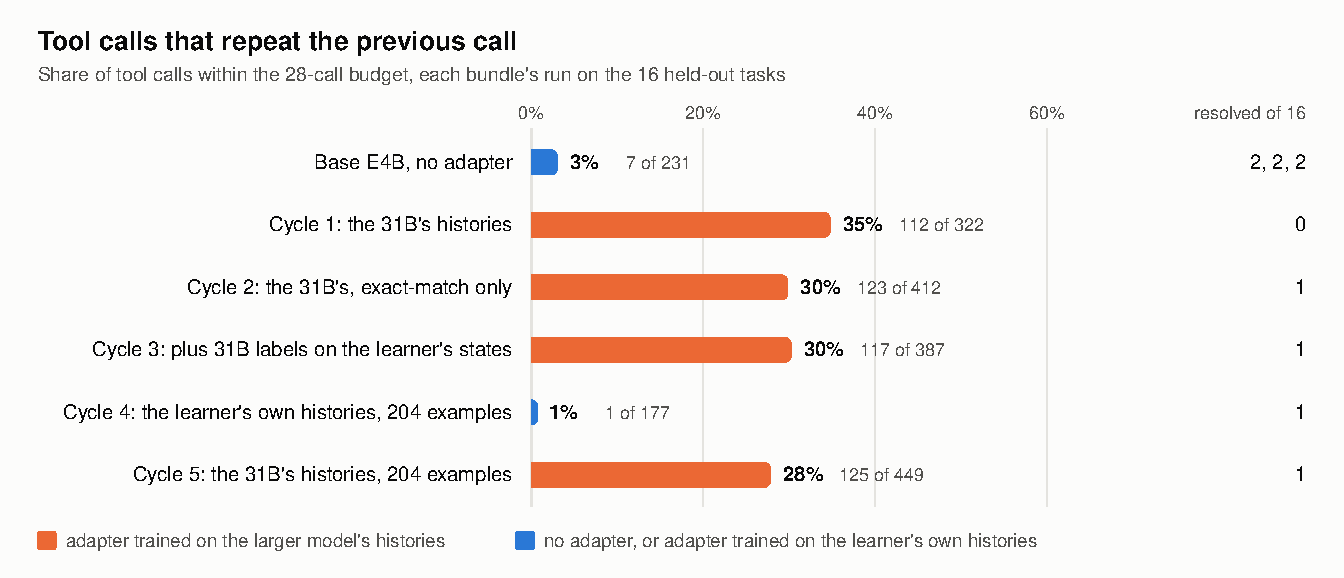
\includegraphics[width=1\textwidth,height=\textheight]{P1-repeat-by-cycle.pdf}
\caption{Repeat rate per bundle on the held-out tasks.}
\end{figure}

\subsection{Cycles 1 and 2: the teacher's
histories}\label{cycles-1-and-2-the-teachers-histories}

The cycle 1 adapter fell into repeat loops: 53 of its 322 calls ran
reasoning to the 4,096-token cap (base: 2 of 231). The targets are not
repetitive (1 exact copy in 844 consecutive pairs): loss on the
teacher's histories improved while generation on the agent's own
histories degenerated.

Cycle 2 was pre-registered before cycle 1's arm returned, with the same
data, base, split and rule but only the exact-match examples; alpha 8
and one epoch were set after cycle 1's result and are labelled post hoc.
Ten of its 16 tasks had three or more repeats. Served at half scale
(update norm 1.06) on four training tasks, cycle 1's adapter had largely
stopped looping; cycle 2, smaller still, looped, so strength alone does
not explain it, and nor does the template difference in cycle 1's bf16
examples.

\begin{figure}
\centering
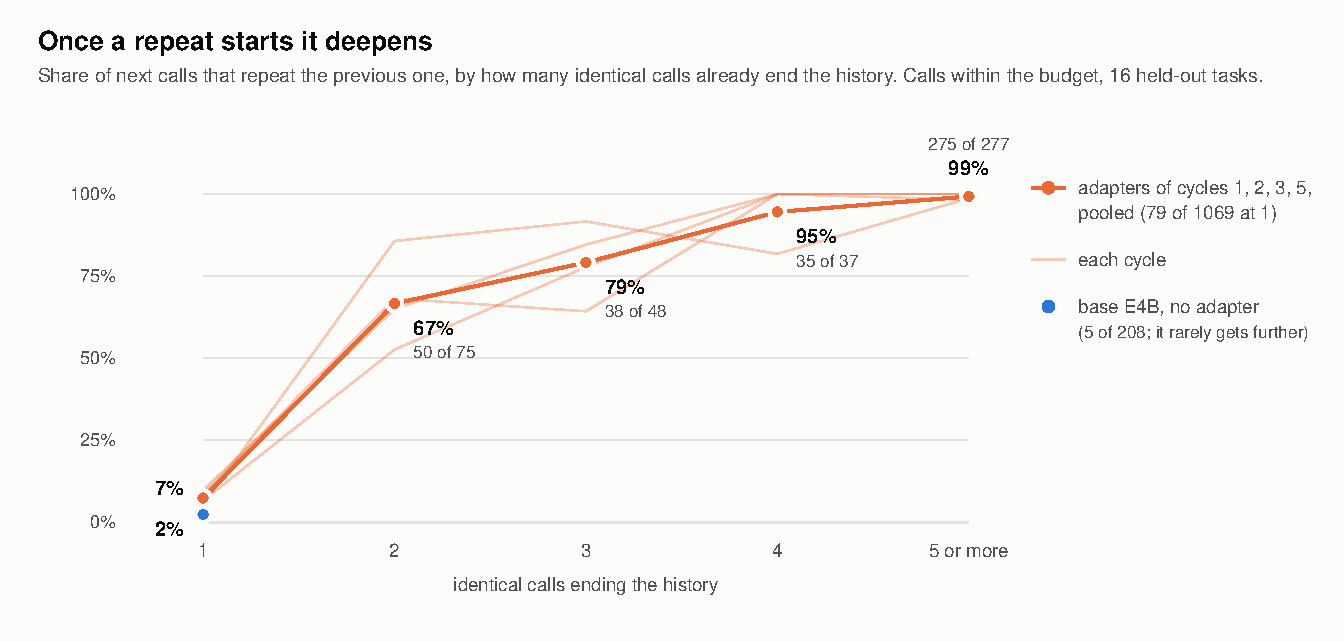
\includegraphics[width=1\textwidth,height=\textheight]{P3-repeat-hazard.pdf}
\caption{The chance of repeating, by how many identical calls already
end the history.}
\end{figure}

The loop deepens itself (Figure 2, post hoc). Pooled over the four
adapters trained on the 31B's histories, an adapter repeats on 7\% of
calls after a non-repeat, on 67\% after one repeat and on 99\% once five
or more identical calls end the history; the base starts a repeat on
2\%. The repeated calls change nothing: reads and commands are 91 to
100\% of them, where six of the base's seven repeats are edit retries,
and the adapters edit about a third as often as the base or less.

The base and cycle 4 never reach the call cap. The four looping adapters
reach it on 8 to 16 tasks and keep asking: 1,719 further calls, most
refused, 81\% repeating the one before. Counted over all calls, their
repeat rates are 54 to 59\%.

\subsection{The instrument: the frontier
swap}\label{the-instrument-the-frontier-swap}

Do the adapter's weights make it repeat whatever its history, or does a
history full of repeats make any E4B repeat? Cut a recorded history
before model call \emph{k}, hand it to another executor and ask for the
next call only: no tool runs. This is DAgger's query of an expert at the
learner's states {[}4{]}, with token-exact admission and writer crossed
with reader. A signed tool fixed the cuts before any output (31B and
base attempts at calls 4, 8 and 12; adapter attempts at their first
repeat and four calls later), admitting 78 of 145 cut histories, or
prefixes, by exact token count: 23 \emph{looping} ones from adapter
attempts and 55 \emph{clean} ones from 31B and base attempts, all before
the call cap. Each executor gives one greedy and four sampled
completions (temperature 0.2) per prefix; a completion repeats when its
first tool call equals the prefix's last, and edits when it is an edit
or write. Differences are paired, with 90\% intervals from 2,000
task-cluster bootstraps and analysis rules fixed before the run.

\begin{figure}
\centering
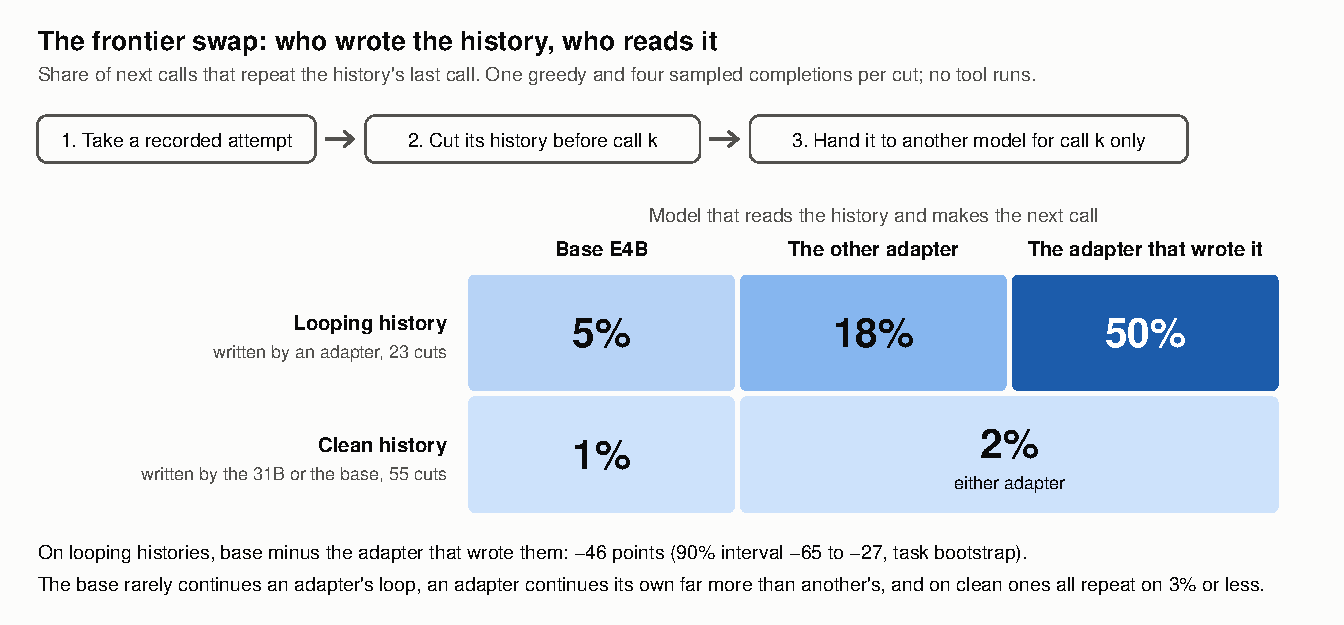
\includegraphics[width=1\textwidth,height=\textheight]{P2-frontier-swap.pdf}
\caption{The frontier swap.}
\end{figure}

On a looping history the adapter that wrote it repeats 50\% of the time,
the other adapter 18\% and the base 5\% (the split by writer is post
hoc); base minus writer is −46 points {[}−65, −27{]}. On clean histories
the adapters differ from base by +2 and 0; none of these is
adapter-written, and in their own rollouts adapters start a repeat on
7\% of calls. The loop needs the adapter and a looping history, and an
adapter's own loop holds it far more than another's. Every looping cut
was adapter-written, from 11 tasks. Admission was uneven, 15 of 30
first-repeat cuts against 8 of 28 four calls later, since compaction
removes long histories, so the looping set leans early. On clean
histories the adapters' next call is an edit 9\% and 11\% of the time
against the base's 36\%.

\subsection{Cycle 3: the expert labels the learner's
states}\label{cycle-3-the-expert-labels-the-learners-states}

One round of expert labelling, a weak test of DAgger {[}4{]}. Cycle 2
was rolled out on 12 of the 52 training tasks; the 31B gave one greedy
next call at each of the 277 states whose rendering matches the served
count; cycle 3 trained on cycle 2's examples plus these; plan, gate and
rule fixed before the rollouts. The expert's labels, by how many
identical calls end the history:

\begin{longtable}[]{@{}lllll@{}}
\toprule\noalign{}
identical calls ending the history & 0 or 1 & 2 & 3 or 4 & 5 or more \\
\midrule\noalign{}
\endhead
\bottomrule\noalign{}
\endlastfoot
states before the call cap & 181 & 4 & 2 & 15 \\
expert repeats & 0 & 0 & 2 & 13 \\
\end{longtable}

The split at the cap is post hoc: 75 of the 277 states follow it, and
there the expert repeats 73 refused calls. Before it, the expert repeats
in 15 of the 17 states ending in three or more identical calls, all from
one task where the learner kept re-running a broken grep. So, on thin
evidence, the expert fails in the states it was asked to correct. The
gate asked for fewer repeats than cycle 2 on looping swap prefixes and
an edit rate on clean ones within 15 points of the base's. Cycle 3
passed the first, 20\% against 30\% (−9 points {[}−17, −2{]}), and
failed the second, 14\% against 36\%. A post-hoc adapter trained without
the 89 rows ending in three or more identical calls, on either side of
the cap, behaved the same, so those labels alone do not keep cycle 3
looping.

\subsection{Cycle 4: the learner's own
histories}\label{cycle-4-the-learners-own-histories}

The base bundle at temperature 0.7 with the clock lifted, six rollouts
over the 52 training tasks: 312 attempts, 34 resolved on 12 tasks. The
render check kept 229 of their examples, and cycle 4 trained from the
base for two epochs on 204. Its gate, fixed before the rollouts, asks
that on clean prefixes it neither repeat more than the base (90\% upper
bound within 5 points) nor edit much less (within 15). It passed: repeat
−0.1 points {[}−1.1, +1.1{]}, edit +1.2 {[}−4.2, +6.4{]}; on looping
prefixes it repeats 2\% against cycle 2's 30\%.

\subsection{Cycle 5: the matched
control}\label{cycle-5-the-matched-control}

Cycle 4 differs from cycles 1 to 3 in size and epochs as well as in its
histories. The control, registered before any draw or run: 204 of cycle
2's exact-match teacher examples, drawn in hash order, cycle 4's
settings, read as looping at a repeat rate of 20\% or more and as not
looping at 10\% or less. It repeated on 125 of 449 calls within budget
(one malformed call did not count against the budget), 28\%, and on 56\%
of all 1,114; 9 of 16 tasks had three or more repeats.

\textbf{What the cycles show.} The four adapters trained on the 31B's
histories, whole, cut to 204 examples or as labels on the learner's
states, fell into repeat loops; the one trained on the learner's own did
not. Update size does not separate them: cycle 4's norm, 0.81, sits
beside the looping 0.89 and 0.91. Cycle 5 rules out example count and
epochs, and cycle 2 the template difference. What remains, once those
are matched, is the source of the histories, which bundles authorship,
style and task coverage. Style is the leading candidate: the loops are
reads and commands, and these adapters edit about a third as often as
the base or less.

\section{The prompt as a lever: two
arms}\label{the-prompt-as-a-lever-two-arms}

Both arms change the prompt, not the weights; both were pre-registered
and run once. \textbf{E4B} submits unchecked fixes: after its last edit,
the last command succeeded in 7 of 16 attempts. Told to check after
every edit, it resolved 3 of 16 against a bar of 4. \textbf{31B} does
not loop; 22 of its 41 unresolved first attempts end at the call cap. It
was told to search once and read 150-line windows. The bar for
resubmission was 33 of 68:

\begin{longtable}[]{@{}lll@{}}
\toprule\noalign{}
31B, first attempts on 68 tasks & window arm & submitted \\
\midrule\noalign{}
\endhead
\bottomrule\noalign{}
\endlastfoot
resolved & 29 & 27 \\
ended at the 28-call cap & 22 & 22 \\
first edit at call, median & 8 & 10.5 \\
read window in lines, median (150 asked) & 61 & 25 \\
\end{longtable}

It followed the instruction in direction and the outcome did not move:
the +2, seven arm-only against five control-only, is inside the ±4 seen
between identical reruns.

\section{Discussion}\label{discussion}

\textbf{What transfers.} Fix the adoption rule against measured rerun
noise before evaluating. Do not read held-out loss alone as progress:
cycle 1 improved it by 28\% while repeating on 35\% of calls, so measure
the repeat rate in free-running rollouts. And probe recorded histories
one call at a time: the swap runs no tools and tested two explanations
in 26 minutes.

\textbf{A hypothesis.} The competition requires one model per submission
{[}15{]}. The swap shows that a history can be handed to another model
for a call, so an agent need not be one model: a cheap model could take
most steps and an expensive one be called on the same history, with no
imitation and so no training mismatch, a cascade {[}9, 10{]} per step.
Our evidence on when to switch is negative: on one task the expert did
not rescue an established loop, and the unadapted learner rarely loops.
We have not run such an agent.

\section{Limitations}\label{limitations}

Sixteen held-out tasks and one attempt per adapter arm: each verdict is
a single draw against a flip rate of one or two in ten. Only the
per-call repeat rates, over hundreds of calls, are well powered, and
calls within an attempt are not independent. One teacher, one learner,
one rank, one seed per cycle, no search. The controlled contrast, cycle
4 against cycle 5, is one draw each, and the two still differ in task
coverage (12 tasks against 30); the teacher differs from the learner in
size and style as well as authorship. We did not test a guard against
identical consecutive calls: bundles admit no code. Cycle 4's rollouts
sample at temperature 0.7, evaluation at 0.2. Cycle 2's settings, cycle
3's second adapter and the count within budget are post hoc and
labelled. Style as the cause is untested, as is the swap on
adapter-written histories before the first repeat. All tasks are public.

\section{Verification and resource}\label{verification-and-resource}

Each step's output names its inputs' digests. The tools that write these
records are signed, and ordering claims rest on the decision log and
Kaggle's version timestamps. Released {[}17{]}: every attempt record and
trace, dataset, adapter, gate, plan and decision record, the decision
log, the prompt-arm bundles, the soundness table, a verifier and the
public key. About 34 L4x4 hours on Kaggle plus 4 Modal A100 hours for
cycle 3.

\section*{References}\label{references}
\addcontentsline{toc}{section}{References}

\begin{enumerate}
\def\labelenumi{\arabic{enumi}.}
\tightlist
\item
  Zelikman, Wu, Mu, Goodman. STaR: Bootstrapping Reasoning With
  Reasoning. NeurIPS 2022; arXiv:2203.14465.
\item
  Gulcehre, Le Paine, Srinivasan et al.~Reinforced Self-Training (ReST)
  for Language Modeling. arXiv:2308.08998, 2023.
\item
  Pan, Wang, Neubig, Jaitly, Ji, Suhr, Zhang. Training Software
  Engineering Agents and Verifiers with SWE-Gym. arXiv:2412.21139. Yang,
  Lieret, Jimenez, Wettig, Khandpur, Zhang, Hui, Press, Schmidt, Yang.
  SWE-smith: Scaling Data for Software Engineering Agents. NeurIPS 2025;
  arXiv:2504.21798.
\item
  Ross, Gordon, Bagnell. A Reduction of Imitation Learning and
  Structured Prediction to No-Regret Online Learning (DAgger). AISTATS
  2011; arXiv:1011.0686.
\item
  Bengio, Vinyals, Jaitly, Shazeer. Scheduled Sampling for Sequence
  Prediction with Recurrent Neural Networks. NeurIPS 2015;
  arXiv:1506.03099.
\item
  Agarwal, Vieillard, Zhou, Stanczyk, Ramos, Geist, Bachem. On-Policy
  Distillation of Language Models: Learning from Self-Generated
  Mistakes. ICLR 2024; arXiv:2306.13649.
\item
  Xu, Liu, Yan, Cai, Li, Li. Learning to Break the Loop: Analyzing and
  Mitigating Repetitions for Neural Text Generation. NeurIPS 2022;
  arXiv:2206.02369.
\item
  Gudibande, Wallace, Snell, Geng, Liu, Abbeel, Levine, Song. The False
  Promise of Imitating Proprietary LLMs. arXiv:2305.15717, 2023.
\item
  Chen, Zaharia, Zou. FrugalGPT: How to Use Large Language Models While
  Reducing Cost and Improving Performance. arXiv:2305.05176, 2023.
\item
  Ong, Almahairi, Wu, Chiang, Wu, Gonzalez, Kadous, Stoica. RouteLLM:
  Learning to Route LLMs with Preference Data. ICLR 2025;
  arXiv:2406.18665.
\item
  Hu, Shen, Wallis, Allen-Zhu, Li, Wang, Wang, Chen. LoRA: Low-Rank
  Adaptation of Large Language Models. ICLR 2022; arXiv:2106.09685.
\item
  Bjarnason, Silva, Monperrus. On Randomness in Agentic Evals. ICLR
  2026; arXiv:2602.07150.
\item
  Gluzdov, Dmitrii. Gemma 4: Measure Before You Tune (now titled ``Gemma
  4: Task Soundness, Serving and Evaluation''). Kaggle notebook, October
  2026.
  \url{https://www.kaggle.com/code/dmitriigluzdov/gemma-4-measure-before-you-tune}.
\item
  Gluzdov, Dmitrii. Gemma 4 Serving and LoRA Verification Kit. Kaggle
  dataset, CC BY 4.0, 2026-10-20.
  \url{https://www.kaggle.com/datasets/dmitriigluzdov/gemma-4-serving-and-lora-verification-kit}.
\item
  Google and Kaggle. Gemma 4 Developer Agent competition: rules and the
  swegemma harness (0.2.11). 2026.
  \url{https://www.kaggle.com/competitions/gemma-4-developer-agent}.
\item
  Henao, W. E. Gemma 4 Agent: Budget-Fit Single Agent. Kaggle notebook,
  October 2026, Apache-2.0.
  \url{https://www.kaggle.com/code/verracodeguacas/gemma-4-agent-budget-fit-single-agent}.
\item
  Lilley, L. gemma-agent records: every attempt record, trace, signed
  item, gate and decision record, the public key and a verifier. Kaggle
  dataset, CC0, 2026.
  \url{https://www.kaggle.com/datasets/leolilley/gemma-agent-records}.
\end{enumerate}

\end{document}
